\documentclass[10pt,aspectratio=169]{beamer}

% to create handouts comment above \document and uncomment the next 3 lines
% \documentclass[10pt, handout, aspectratio=169]{beamer}
% \usepackage{styles/handoutWithNotes} % requires handoutWithNotes.sty
% \pgfpagesuselayout{4 on 1 with notes}[a4paper,border shrink=5mm]

% packages
\usepackage{graphicx}
\usepackage{multicol}
\usepackage{url}

% presentation settings
% custom theme modified from http://www.math.ucdenver.edu/~hbouwmee/resources.php
% must have beamerthemeCU.sty and cu_logo.eps in styles directory
\usepackage{styles/beamerthemeCU}
\setbeamertemplate{section in toc}[sections numbered]
% \setbeamertemplate{caption}{\raggedright\insertcaption\par} % don't display Figure for each fig
\setbeamertemplate{caption}[numbered]

% image path
\graphicspath{ {images/} }

% bibliography settings
\setbeamertemplate{bibliography item}{} %remove the icon
%remove line breaks
\setbeamertemplate{bibliography entry title}{}
\setbeamertemplate{bibliography entry location}{}
\setbeamertemplate{bibliography entry note}{}
\setbeamertemplate{bibliography item}{\insertbiblabel} % display item numbers

% presentation information
\title{PlanetiQ Pyxis: Kalman Filter}
\institute{University of Colorado Boulder}
\author{Rane Brown}
\date{\today}

% start of presentation
\begin{document}

\begin{frame}[t,plain] % t = top align, plain = no header or footer
    \titlepage
\end{frame}

\begin{frame}[t]{Table of Contents}
    \begin{center}
        \vspace{-2em}
        {\Large \textbf{\underline{Outline}}}
        \vspace{1em}
    \end{center}
    \begin{multicols}{2}
        \tableofcontents
    \end{multicols}
\end{frame}

\section{Objectives}%-------------------------------------------------------------------------------

    \begin{frame}{Independent Study Objectives}
        \begin{itemize}
            \item Basic understanding of the Pyxis project and the importance of the Kalman filter
            \item Create unit tests for all crucial functions used by the Kalman filter
            \item Integrate C port of navigation filter into Pyxis code framework
            \item Analysis of various matrix libraries with pros and cons of each
            \item Debugging of Kalman filter upon integration into overall system
            \item Testing, tuning, and profiling of Kalman filter
        \end{itemize}
    \end{frame}

\section{Big Picture}%------------------------------------------------------------------------------

\subsection{Pyxis}
    \begin{frame}{Purpose of Pyxis Project}
        \begin{itemize}
            \item Pyxis is a satellite instrument designed to collect GNSS signals to make measurements of the Earth's atmosphere via "Radio Occultation"
            \item The Pyxis receiver design and implementation is a joint effort between the University of Colorado and Space Sciences and Engineering of Boulder
            \item Currently, the major software components that will be used on the satellite are under development
        \end{itemize}
    \end{frame}

\subsection{Radio Occultation}
\begin{frame}{What is Radio Occultation?}
    \begin{columns}
        \begin{column}{0.6\textwidth}
            \begin{itemize}
                \item A radio signal transmitted by a GPS satellite in medium Earth Orbit is bent as it travels through the Earth's atmosphere
                \item Signal is then received by a satellite in low Earth orbit (LEO) less than about 1,200 miles above the planet
                \item The bending angle can be used to calculate the atmospheric density, which can be used to calculate temperature, pressure, humidity and electron density.\cite{planetiQ:2016}
            \end{itemize}
        \end{column}
        \begin{column}{0.4\textwidth}
            \begin{figure}
                \centering
                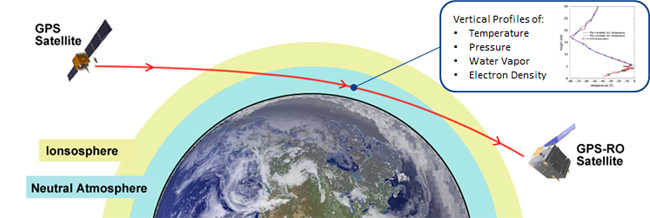
\includegraphics[width=6cm]{ro}
                \caption{Radio Occultation\cite{planetiQ:2016}}
            \end{figure}
            \end{column}
    \end{columns}
\end{frame}

\begin{frame}{Position and Velocity of RO Satellite}
    \begin{itemize}
        \item In order to utilize the radio occultation technique it is necessary to have \underline{very} accurate estimations of the RO satellite position and velocity
        \item To obtain the desired accuracy a Kalman filter is implemented in software
        \item The models used in software and the satellite observations use different coordinate frames i.e.\ ECEF and ECI
            \begin{itemize}
                \item It is necessary to have the ability to easily convert between these different coordinate frames on a frequent basis
            \end{itemize}
    \end{itemize}
\end{frame}

\subsection{Kalman Filter}
    \begin{frame}{What is a Kalman Filter?}
        \begin{columns}
            \begin{column}{0.9\textwidth}
                \begin{block}{Definition}
                    \begin{itemize}
                        \item An algorithm that combines physical models and sequential observations to obtain an estimation of a state at a given time.
                        \item The filter uses a recursive formula and aims to minimize the mean of the squared error \cite{welch:1995}
                    \end{itemize}
                \end{block}
            \end{column}
        \end{columns}
    \end{frame}

\subsection{Coordinate Frames}
    \begin{frame}{ECEF and ECI}
        \begin{columns}
            \begin{column}{0.6\textwidth}
        \begin{block}{Earth-centered, Earth-fixed}
          A $(X,Y,Z)$ coordinate system where the point $(0,0,0)$ is defined as the center of mass of the Earth. The axes are also aligned in a fixed position with respect to the Earth's surface i.e. the earth does not rotate about an axis\cite{leick:2004}
        \end{block}
        \begin{block}{Earth-centered inertial}
          A coordinate system with the center defined as the center of mass of the Earth. The $(X,Y,Z)$ axes are fixed in place and the Earth rotates around the $Z$ axis unlike ECEF coordinates.\cite{Ashby:2004}
        \end{block}
            \end{column}
            \begin{column}{0.4\textwidth}
                \begin{figure}
            \centering
                    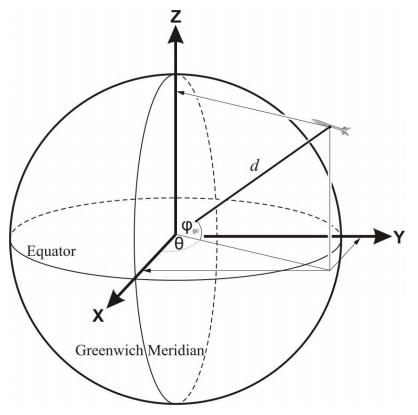
\includegraphics[width=0.3\textwidth]{ECEF}
            \caption{ECEF Coordinates\cite{polecats:2016}}
                \end{figure}
          \begin{figure}
            \centering
            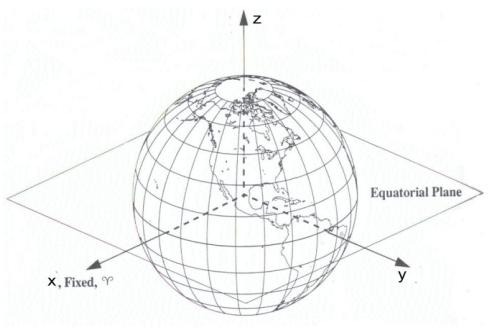
\includegraphics[width=0.4\textwidth]{ECI}
            \caption{ECI Coordinates\cite{polecats:2016}}
          \end{figure}
            \end{column}
        \end{columns}
    \end{frame}

\section{Code}%-------------------------------------------------------------------------------------

\subsection{Approach}
    \begin{frame}{Approach}
        \begin{itemize}
            \item Matlab Navigation filter written by Daehee Won provides a baseline for desired output
            \item Most functions were ported to C as part of the DLA Research Program
            \begin{itemize}
                \item Major structural changes necessary
                \item Pyxis project uses threading and relies on communication between modules
                \item Current C port still provides a good starting point
            \end{itemize}
            \item Incrementally write functions and utilize unit test framework to verify results
        \end{itemize}
    \end{frame}

\subsection{Check Framework}
    \begin{frame}{Unit Tests}
        \begin{block}{}
        {{\Huge``} The incremental test/code approach provides three main benefits to the developer:
            \begin{enumerate}
                    \item Because the unit tests use the interface to the unit being tested, they allow the developer to think about how the interface should be designed for usage early in the coding process.
                    \item They help the developer think early about aberrant cases, and code accordingly.
                    \item By providing a documented level of correctness, they allow the developer to refactor aggressively.
                \end{enumerate} {\Huge''}}\cite{check:2016}
        \vskip5mm
        \end{block}{}
    \end{frame}

\subsection{Git}
    \begin{frame}{Importance of Git}
        \begin{itemize}
            \item Pyxis project is setup as an organization on github
            \item Each person works on separate branches and opens ``pull requests'' to merge code back onto the master branch
            \item Provides important version control and separation of different modules
            \item Cross platform compatibility
        \end{itemize}
    \end{frame}

\subsection{Compatibility}
    \begin{frame}{Compatibility between C and Matlab}
        The original Kalman filter was written in Matlab and the output is verified as correct.
        \begin{itemize}
            \item This provides a good baseline for testing the output of the C port
            \item It is difficult to convert data into a format the can be read by C for testing
                \begin{itemize}
                    \item The easiest approach was found to output the Matlab data to a text file
                    \item Use fscanf to read in data
                    \item Approach works but is cumbersome and can be prone to errors
                \end{itemize}
            \end{itemize}
    \end{frame}

\subsection{Matrix Libraries}
    \begin{frame}[t]{Linear Algebra}
        The Kalman filter heavily utilizes linear algebra and matrix operations. This fact made obtaining a verified and function rich linear algebra library a priority.\\
        \vspace{0.5em}
        \textbf{Options:}
        \begin{description}
            \item[Meschach] Standalone library that is fairly fast and provides the needed functionality. Matrices are built using data structures that allow resizing.
            \item[CBLA] C implementation of the BLAS (Basic Linear Algebra Subprograms) library which was originally written in Fortran. Widely used and well tested but most functions are low level and meant to be used as a base for a separate library.
            \item[GSL] The GNU Scientific Library: uses BLAS as a base and provides over 1000 functions.
            \item[Utils] \alert{Custom library developed for the Pyxis project - most functions needed for the Kalman filter are already present.}
        \end{description}

    \end{frame}

\subsection{Testing}
    \begin{frame}{Testing and Debugging}
        \begin{columns}
            \begin{column}{0.6\textwidth}
        \begin{itemize}
            \item Unit tests for basic functionality
            \item Matlab Navigation Filter as baseline
            \item Removal of redundant code
            \item Utilization of data structures
            \item Comparison to truth
        \end{itemize}
            \end{column}
            \begin{column}{0.4\textwidth}
                \begin{figure}
            \centering
                    
\includegraphics[width=1\textwidth]{bug}
            \caption{Debugging\cite{bug:2013}}
                \end{figure}
            \end{column}
        \end{columns}
    \end{frame}

\subsection{Status}
    \begin{frame}{Future Work}
        \begin{itemize}
            \item Real-time testing
            \item Determine time filter takes to run (as expected?)
            \item Tuning and optimization of configurable parameters
            \item Incorporation of Kalman filter into threaded Pyxis framework
        \end{itemize}
    \end{frame}

\section{Conclusion}%--------------------------------------------------------------------------
    \begin{frame}{Lessons Learned}
        \begin{enumerate}
            \item Care must be taken to not create circular dependencies when working on projects with many separate files and headers
            \item Doxygen is a useful tool for documenting code - it helps provides a better understanding of how a function is designed
            \item Working on a large scale software project is challenging and communication is an essential part of the process
            \item Writing code and debugging/testing can take more time than expected and planning for this eventuality can provide the needed time buffer
        \end{enumerate}
    \end{frame}

\section{References}%-------------------------------------------------------------------------------

    \begin{frame}[t]{References}
            \footnotesize
            \bibliographystyle{ieeetr} % must come before bib filename
            \bibliography{bibliography/kal_ref}
    \end{frame}

\end{document}
